[Here I describe the overall characteristics and limitations that a VLC system should present according to my findings, identify the variables involved and the set of parameters necessary for it to work\\
This chapter should provide a useful starting point for whoever plans to implement one in practice]\\
What does one need to make his own VLC system?\\

Structure of a VLC system: logical layer, control layer, physical layer. Analysis and characteristics of the three.

[Here I describe the system that I prototyped, characteristics of hardware and software]\\
\[It could be shorter, might move some stuff to the previous chapter\]

\subsection{Architecture}

The system is composed of two main modules: a transmitter module, and a receiver.
The transmitter module takes some input, encapsulate it and encodes it as oscillations in light intensity, through the control of a light emitter.
The receiver side interprets the light variations, reconstructing the light stream back into messages and forwarding it to the consumer of the information. 
Each module includes different components, listed in detail.

\begin{figure}
\centering
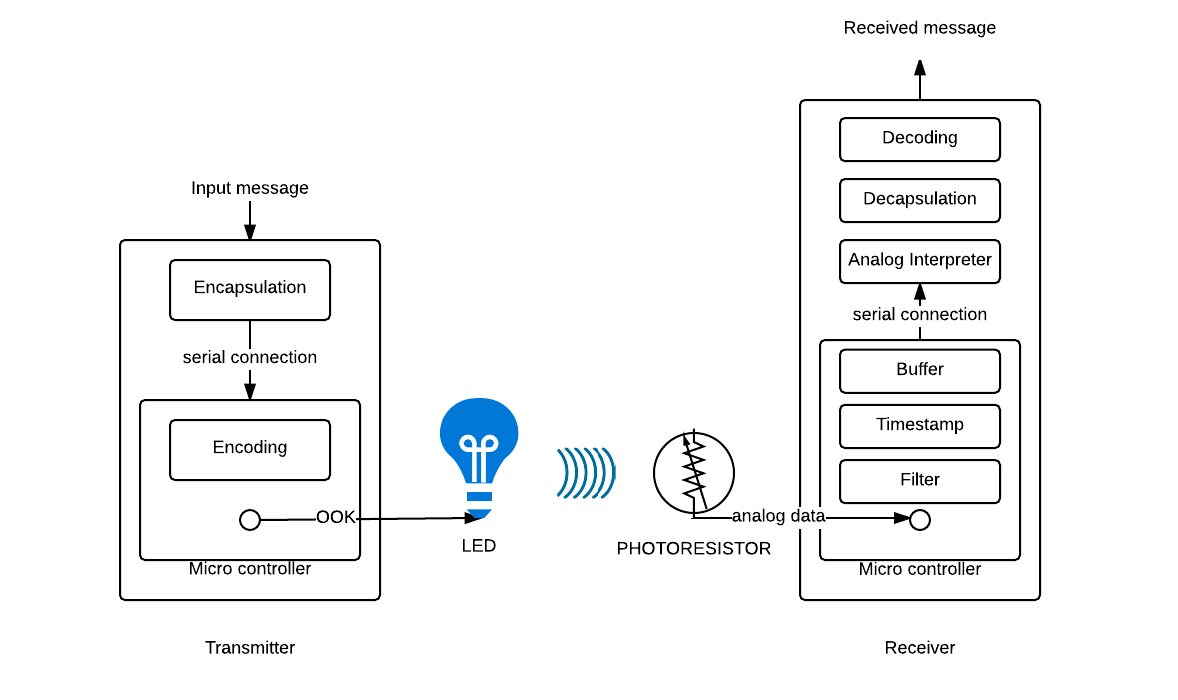
\includegraphics[height=200px]{img/sysover}
\label{fig:sys over}
\caption{System architecture.}
\end{figure}

\subsubsection{Transmitter}
Transmission starts from a terminal, where a client can input messages as strings. These are then encapsulated into Protocol Data Units (PDUs) and sent to a micro controller through a serial connection.
In this case, the micro controller that was used for transmission is an Arduino board.
\footnote{TODO find a place for this: One aspect to consider in implementing this passage is that the serial buffer has a limited size of 64 bytes in most Arduino boards, so it's important to keep the serial communication as light as possible to avoid overflow. In most cases, it's possible to encode a char into one single 8-bits byte, but not all the programming languages implement this automatically.
The system described in this paper was implemented using Python 2.7, which uses dynamic types and therefore doesn't have a specific type for \textit{chars}. In Python, strings have an overhead of 37 bytes, plus one byte for every character in the string, this would result in a very heavy serial transmission for just a few characters. Characters need to be converted in single bytes before sending them. }

The board encodes the received bytes into Manchester Code, and then controls the light signal by switching on and off the emitter accordingly.
A light emitting diode is the furthest end of the transmitter module. In early stages prototyping, this consisted of a single low power LED directly connected to the board and powered by it, while in the final system it was replaced by a commercial LED bulb. The bulb is powered by an external power source (mains electricity), and controlled by the board through a switcher. 

\subsubsection{Receiver}
Sending light signals is not too complicated, what really is the core of the project is to read such signals and interpret the sensor data correctly.
The signal is received by a photodiode,  or light sensor, read by a second micro controller as analog input.
On the board, values are software-filtered to reduce noise, and sent to the receiving terminal with a timestamp.
The board and the terminal are connected through a serial connection.
Some controllers could read directly analog input and perform the remaining processes to interpret the signal, with enough computational power.\\ For this application, the final terminal is a Raspberry Pi, since it has a good power/size ratio for the designed purpose and allows a simpler prototyping process. The micro controller in between the two is necessary to read and forward analog data from the sensor.\\
On the final terminal, the variations of sensory data are interpreted as sequences of digital 0s and 1s, finally decapsulated and decoded back into a message.

\subsection{Hardware}
[list of components and physical properties/characteristics]\\
Hardware components: TODO list models and stuff
\begin{enumerate}
\item Micro controllers:
\begin{enumerate}
\item Genuino Uno for the transmitter
\item Arduino Yun for the receiver
\end{enumerate}
\item low power LED
\item commercial LED bulb, 240 V, ...
\item terminals:
\begin{enumerate}
\item laptop computer
\item Raspberry Pi
\end{enumerate}
\item photo resistor
\item Solid State Relay
\end{enumerate}
\textbf{Characteristics of the LED}:\\
low power, 5V \\
average time for changing LED state at rest. \\
turning ON from OFF (stable)
turning OFF from ON (stable) \\
%times of 65% growth (avg) 3.48200000001
%times of 73% growth (65% of 1s) 4.52000000001
%times of 80% growth (96% of 1s) 6.122
%times of full growth 49.03
%times for decrease to 35% (avg 0s) 4.25999999999
%times for decrease to 45% (65% of 0s) 3.37999999999
%times for decrease to 58% (96% of 0s) 2.50999999999
%times of full decrease  62.84
As can be seen in fig. \ref{fig:txpeak}, during transmission the brightness achieved from the LED used for testing is not at 100\%. In the figure, after the transmission terminates the LED reaches maximum brightness at the far right of the graph.\\ Table \ref{table:warmup} shows the physical characteristics of the LED concerning times to reach specific levels of brightness. Times to reach a level of brightness are calculated starting from the opposite full state (time to reach a local maximum from completely OFF, or a local minimum from completely ON).
Meaningful levels that are considered are:
\begin{enumerate}
\item the maximum and minimum level of brightness of the LED
\item the level at which the average $\mu$ peak is during transmission is, either local minimum for a 0 or 00 or local maximum for a 1 or 11
\item the level at which $\mu +- \sigma$ of the sampled peaks are during transmission, this represents about 65\% of the peaks
\item the level at which $\mu +- 2\sigma$ of the sampled peaks are during transmission, this represents about 96\% of the peaks
\end{enumerate}
%Also, something to think about is that a peak in transmission is never at the same height of a peak during no transmission, but it's at some percentage lower produce statistics about that, average peak in transmission vs. average height level not in transmission What is really meaningful is how fast can I get to transmission peak from 0, rather than to 1 peak, because that's how much time I need to start the transmission(something like: transmission 1s come at 60\% the  maximum brightness, while transmission 11s come at 80\%)\\

\begin{tabular}{l c c c r}
\hline
peak & brightness ON & turning ON & brightness OFF & turning OFF \\
$\mu$ & 65\% & 3.4 ms & 35\% & 4.2 ms \\
$\mu +- \sigma$ ( 65\% )& 73\% & 4.5 ms & 45\% &  3.4 ms \\
$\mu +- 2 \sigma$ ( 96\%) & 80\% & 6.1 ms & 58\% & 2.5 ms \\
 - & 100\% & 49.0 ms & 0\% & 62.8 ms \\ 
\hline
\label{table:warmup}
\end{tabular}
\newline \newline \newline
\textbf{Characteristics of the bulb}:\\ 
dimmable, warmup time unknown\\
flicker rate, again, unknown\\
TODO\\
\newline
\textbf{Characteristics of the switcher (SSR)}:\\
unknown, TODO\\

\begin{figure}
\centering
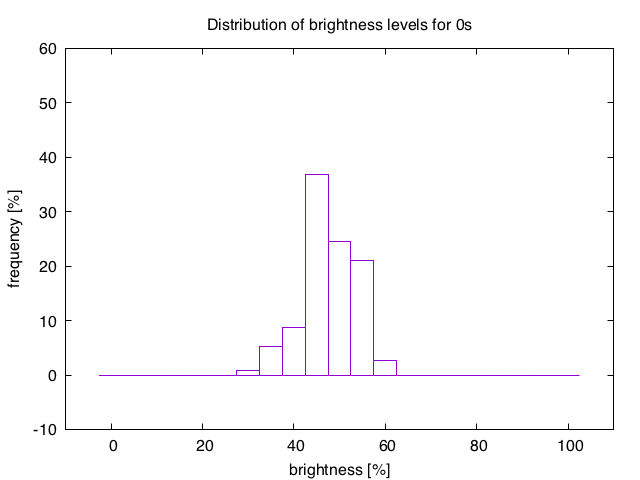
\includegraphics[height=100px]{img/hist0}
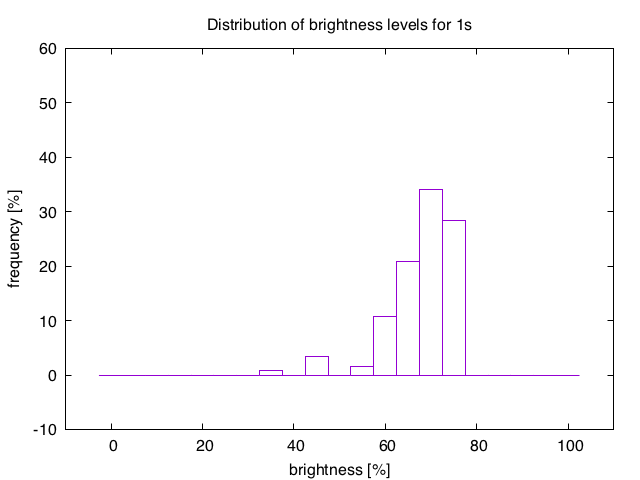
\includegraphics[height=100px]{img/hist1}
\label{fig:histopeaks}
\caption{Brightness levels during transmission, brightness of 0s to the left, 1s to the right. }
\end{figure}

\begin{figure}
\centering
\includegraphics[height=180px]{img/warmup}
\label{fig:warmup}
\caption{LED warmup time}
\end{figure}

flicker rate? meaning the maximum amount of times the LED can change it's state in a given time unit. I can't measure this with the current receiver, it would be too fast (more than 1 kHz, but I can't know how much more, since the receiving rate is of about 1.2 kHz). \\

\subsection{Transmission}
[encoding, interval, rates, reading]

\begin{figure}
\centering
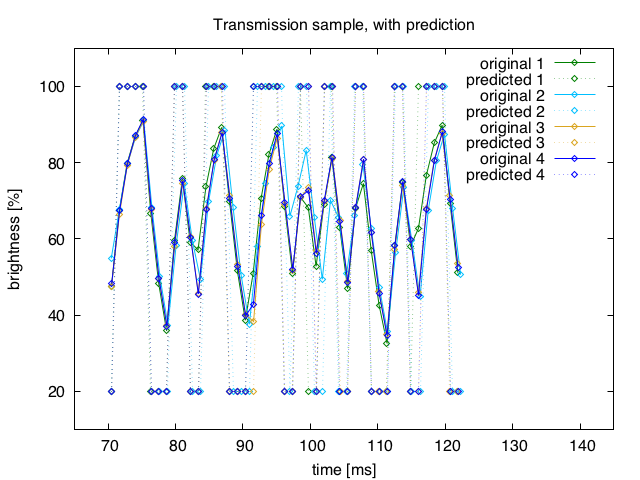
\includegraphics[height=180px]{img/sample}
\label{fig:sample}
\caption{signal sample, analog in green, digitalised in purple.}
\end{figure}

\subsubsection{Transmission rate}
The signal is encoded using manchester coding {ref} which converts each binary 1 into a 01 and each binary 0 into a 10.
Each single symbol is forced to last for 2 ms before the transmitter board sends out the next, for ensuring a better reception.
The transmission rate would therefore be at best of 500 bits/s in theory, in the case where the activity of the micro controller pays no role.
This value was experimentally measured to be slightly smaller, at around 450 bits/s. 

TODO remember to include also baud rates

\subsubsection{Reception rate}
On the reception side, no time boundaries are set, meaning that the reception happens as fast as the board is ready to retrieve values from the sensor.
 the average reception rate is of about one value every 0.833 ms  (~1200 bits/s)
 
 \subsubsection{Reading the signal}
[ shape, noise, machine learning difficulties, final resolution ]\\
A key part of this project is to convert analog sensor data representing light variations into binary code.
Fig. \ref{fig:sample} shows a sample of transmission. The green line represents the original values from the light sensor, while the purple line is a reconstruction of what the digital transmission would look like. Manchester encoding allows transmission to only have two kinds of peaks, either representing single bits, like a 1 or a 0, or two bits of the same kind.
Having a longer sequence of identical symbols would be impossible with this encoding.\\

Multiple attempts have been made to design an algorithm that would interpret this sequences of values into binary data.\\
The first version of it made use of Machine Learning techniques to train a model with training data, "teaching" a classifier what kinds of data and results one would expect in this application. The data was taken in different circumstances of ambient light interference, with different messages sent and at different times.
Multiple classifiers were tested, with a maximum success rate of about 75\%. The classifiers included NaiveBayes, RandomForest, AdaBoost and ArtificialNeuralNetworks, all with comparable results.\\
There were major difficulties with this approach. For starters, there were problems identifying the labels to train these models, namely the classes or categories where the data would belong.
Initially, the four categories were "1", "0", "11", and "00". The basic idea is that given a sequence of values it should fall in one of these four classes. The problem was though that single bits and double bits have different sizes in amount of values that form them. This is also called the number of features.\\
Most standard modules for machine learning require the same number of features for all the labels.\\
In order to get around this rule, the labels became "10", "01", "11", and "00". Eventually, also these labels were produced by different numbers of features. Other combinations were tried, and eventually all leading to the same result. 
One way to get around this problem was to have a fixed number of features, but big enough to include all the possibilities. Samples smaller than this maximum amount (virtually all of the samples) would be filled up with blank values until they reached the intended size.\\
Another way would be to train a classifier for each specific number of features that may occur. In this case, the amount of classifiers needed would be around 4, for number of features ranging between 7 and 10.
The downside of this approach is that each classifier becomes very specific to a restricted set of the training data, potentially loosing track completely of certain labels.\\
The final setup for machine learning prediction used the labels "101", "100", "011", "110", "001", "11", "00", "10", "01", scaling of the features and larger sample size to be filled up with blanks. This produced overall the best results for the machine learning approach, but never above 80\% success rate.\\
A second downside to this approach would be that when receiving values from the sensor in real time, one would need to 
keep a moving window  of the size of the number of features and try to obtain a prediction from the classifier each time.
This might likely slow down the reading process.\\

These poor results ultimately led to a change of approach for reading the data. 
Just looking at fig. \ref{sample} it's pretty straightforward to see that the high peaks represent 1s and the low peaks represent 0s. 
By setting some rules, a custom classifier could predict a result without the need to be trained with sample data.
In particular, the classifier analyses sequences of values, trying to find sequences that are either monotonically increasing or monotonically decreasing.
Also a noise factor has to be taken into account, in this way small enough variations are not considered.
As mentioned before, there are only two kinds of peaks in the sequences, either single or double peaks.
Therefore, it's of critical importance to be able to distinguish the two cases. One criteria that was originally deployed for this was to count the number of values that progress in the same direction, either up or down. This was later changed to the more precise criteria of duration of such sequences, and this is the reason why for each value a timestamp is included representing the time of reception for that specific value.\\ TODO stats about reception rate, std deviation.\\
With this in mind, the algorithm has been developed to very simply count the duration of either monotonically increasing or decreasing sequences of values, and produce a prediction when the direction changes, based on such duration.
This technique performs particularly well in this application, producing up to 100\% success rate in certain cases.
 Runtime wise, the algorithm takes constant time for each value that that is received, and may or may not produce a result.
A simplified version of the algorithm can be found in fig. \ref{code}.
\begin{figure}
\centering
\begin{lstlisting}[language=Python, frame={}]
	def feed(self, time, value):
		pred = None
		
		# staying
		if abs(value - self.prev) <= self.epsilon:
			pass

		#going down
		elif value <= self.prev: 
			if self.direction: # up	
				pred = self._predict(time)

		# going up
		elif value > self.prev: 
			if not self.direction: # down
				pred = self._predict(time)

		self.prev = value
		return pred
		
	def _predict(self, time):
		m = self.direction
		delta = time - self.seqstart
		pred = '-'
		
		if delta >= self._doubletime:
			pred = '11' if m else '00'
		else:
			pred = '1' if m else '0'

		self.direction = not self.direction
		self.seqstart = time
		return pred
\end{lstlisting}
\label{code}
\caption{Simplified algorithm for signal interpretation (Python 2.7).}
\end{figure}

\subsection{Protocol}
As can be seen the rates of transmission and reception in this prototype system are not very high, if compared to average wireless transmission speeds, which are measured in Mbps.
Transmission in visible light is also exposed to a high degree of uncertainty, depending on parameters like distance, maximum brightness, interference, noise, and so on.
In this prototype, communication is only established in one direction, which additionally increases the treat of getting wrong results.
In order to compensate all this aspects, an effort to strengthen the success rate has been made by structuring the communication into a very basic protocol.
Each PDU is included between two single bytes: STX, that indicates the start of a message, and a byte ETX which indicates its end. These two are bytes 0x02 and 0x03 respectively. To avoid that the reader assumes an ETX byte wrongfully while reading the message, a length byte LEN is also included in the header of the PDU, to specify the length of the message in bytes.
Additionally, each PDU is restrained to have a maximum size, and longer messages need to be split into more PDUs.

\subsubsection{Additional fields}
Increasing the functionalities or complexity of the system, additional parameters in the PDU might result useful if not necessary. 
Imagining a scenario with multiple receivers of messages broadcasted through light in a unilateral way, a receiver field could be added to the PDU. Also, it would be wise to perform encryption on the PDUs, in a way that only the intended receivers would be able to read the message directed to them.
Establishing 2-way communication would also require more steps. 2-way communication would be a very good way to ensure correctness of the transmission. For this, at least 2 more parameters seem necessary: a sequence number to identify the packet, and a checksum to check correctness of the received message.
A header for visible light communication doesn't require many parameters since it's likely to be the very last end of a communication process. Since it's mainly short distanced, it doesn't need any routing parameters as it would in big networks. 

\begin{figure}
\centering
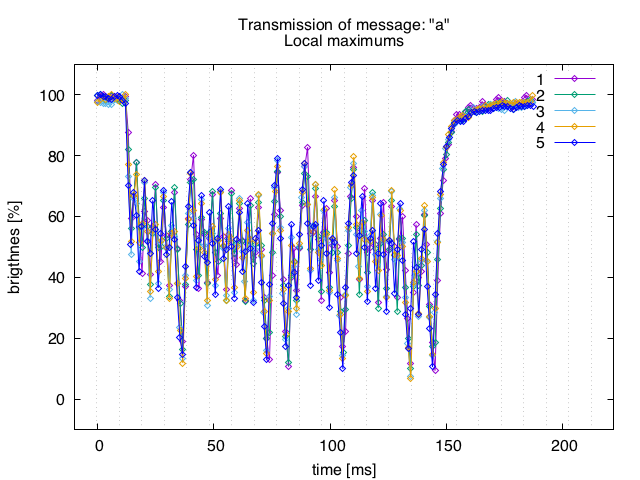
\includegraphics[height=180px]{img/transmission}
\label{fig:txpeak}
\caption{Example of transmission of message "a", including STX, ETX and LEN fields}
\end{figure}



